\section*{Platinsponsor und Aussteller}
\begin{center}
  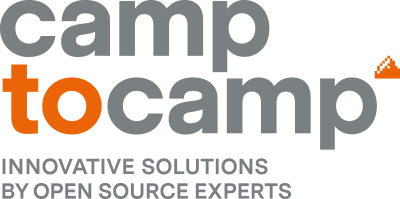
\includegraphics[width=0.7\textwidth]{001_camptocamp_logo.png}
\end{center}
Camptocamp gehört zu den führenden Dienstleistern im Bereich Open-Source-GIS und ist in vielen unterschiedlichen Open-Source-Communitys stark engagiert.

Unsere Dienstleistungen stützen sich auf 20 Jahre Erfahrung in der Umsetzung von innovativen GIS-Lösungen für Behörden und Unternehmen und erlauben einen hochwertigen und individuellen Service. Das Besondere an Camptocamp sind die hochqualifizierten Mitarbeiter und ihr großes Engagement im "`Ökosystem"' der eingesetzten Open-Source-Software-Lösungen, indem sehr enge Beziehungen zu den Herstellern der jeweiligen Produkte gepflegt werden.

Um die oft anspruchsvollen Projekte umzusetzen, erstellt Camptocamp individuelle Lösungen, die auf den am besten geeigneten und fortschrittlichsten Open-Source-Technologien basieren. Camptcamp ist in München, Lausanne, Olten, Paris und Chambéry vertreten und bietet neben Lösungen im GIS-Bereich auch eine große Expertise im den Bereichen ERP (Enterprise-Resource-Planning) und IT-Infrastruktur-Lösungen.
